\documentclass[border=4pt,crop=true]{standalone}
\usepackage{pgfplots}
\pgfplotsset{compat=1.18}

\begin{document}
\begin{tikzpicture}
  \begin{axis}[
    width=10.5cm,
    height=5.8cm,
    xmode=log,
    ymode=log,
    xmin=1e-1,
    xmax=1e2,
    ymin=1e-2,
    ymax=1e2,
    axis lines=left,
    xlabel={$\omega/\omega_c$},
    ylabel={$R_C/R$},
    xtick={1e-1,1,1e1,1e2},
    xticklabels={$0.1$,$1$,$10$,$100$},
    ytick={1e-2,1e-1,1,1e1,1e2},
    yticklabels={$0.01$,$0.1$,$1$,$10$,$100$},
    grid=both,
    minor tick num=1,
    tick label style={font=\small},
    label style={font=\small},
    every axis plot/.append style={thick},
  ]
    \addplot[domain=1e-1:1e2,samples=300] {1/x};
    \addplot[gray,dashed] coordinates {(1,1e-2) (1,1e2)};
    \addplot[gray,dashed] coordinates {(1e-1,1) (1e2,1)};
    \node[anchor=south west,font=\small] at (axis cs:1,1) {$\omega_c=\dfrac{1}{RC}$};
    \node[anchor=south west,font=\small] at (axis cs:0.13,9) {$R_C\gg R$};
    \node[anchor=north east,font=\small] at (axis cs:40,0.03) {$R_C\ll R$};
  \end{axis}
\end{tikzpicture}
\end{document}
